\documentclass{standalone}
\usepackage{tikz}
\usetikzlibrary{patterns, positioning}


\begin{document}
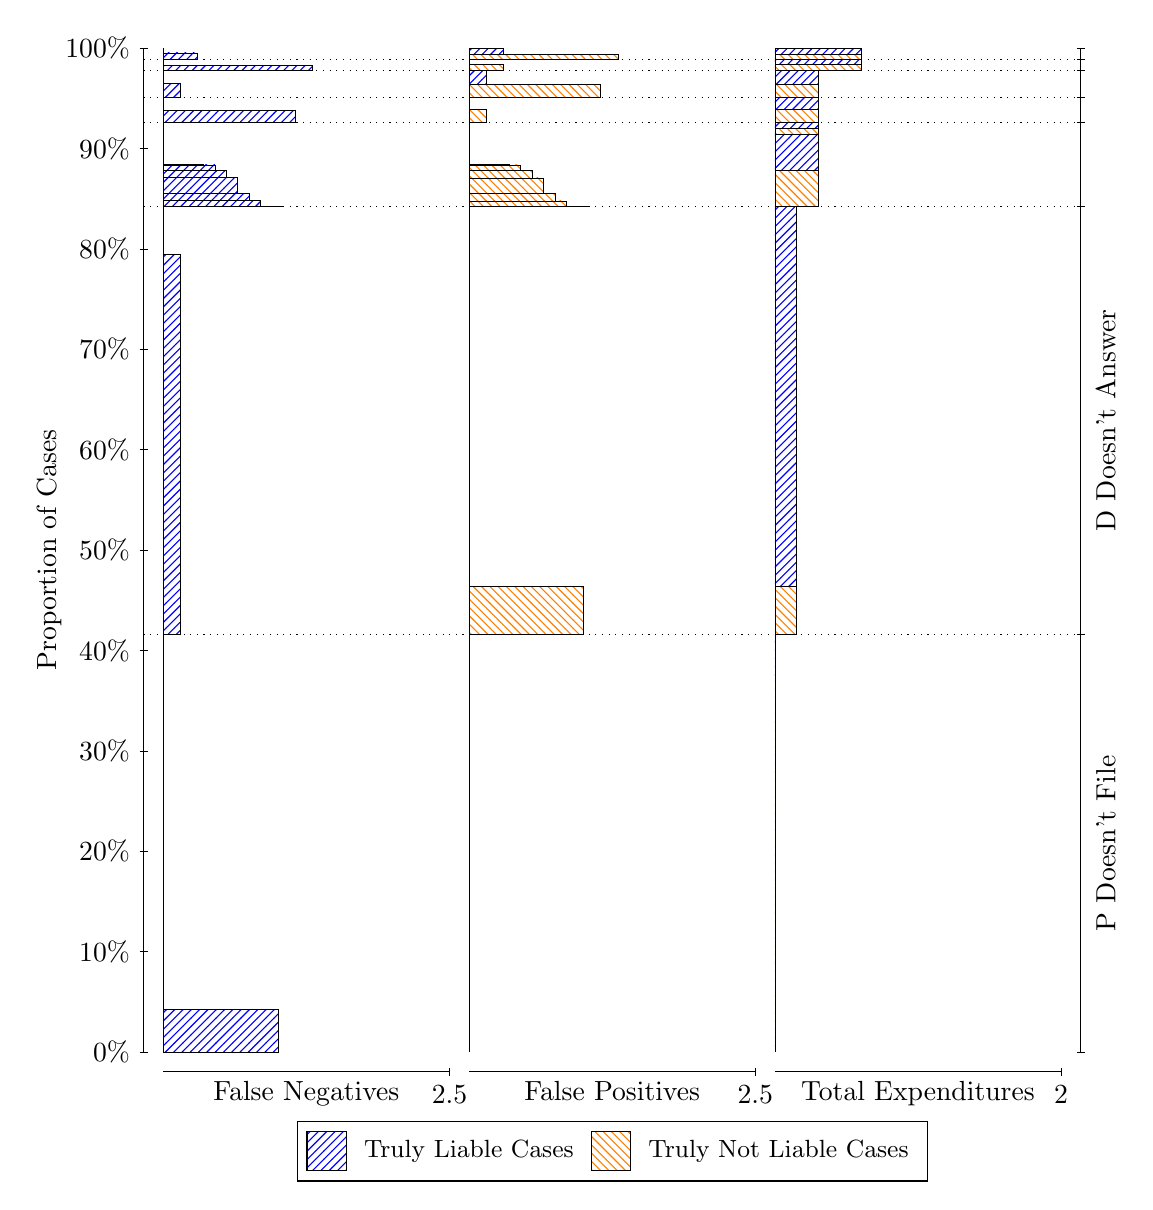
\begin{tikzpicture}
\draw[black, very thin] (1.5,1.75) -- (1.5,14.5);
\node[rotate=90, text=black, anchor=center] at (0.3, 8.125) {Proportion of Cases};
\draw[black, very thin] (1.45,1.75) -- (1.55,1.75);
\node[text=black, anchor=east] at (1.45, 1.75) {0\%};
\draw[black, very thin] (1.45,3.025) -- (1.55,3.025);
\node[text=black, anchor=east] at (1.45, 3.025) {10\%};
\draw[black, very thin] (1.45,4.3) -- (1.55,4.3);
\node[text=black, anchor=east] at (1.45, 4.3) {20\%};
\draw[black, very thin] (1.45,5.575) -- (1.55,5.575);
\node[text=black, anchor=east] at (1.45, 5.575) {30\%};
\draw[black, very thin] (1.45,6.85) -- (1.55,6.85);
\node[text=black, anchor=east] at (1.45, 6.85) {40\%};
\draw[black, very thin] (1.45,8.125) -- (1.55,8.125);
\node[text=black, anchor=east] at (1.45, 8.125) {50\%};
\draw[black, very thin] (1.45,9.4) -- (1.55,9.4);
\node[text=black, anchor=east] at (1.45, 9.4) {60\%};
\draw[black, very thin] (1.45,10.675) -- (1.55,10.675);
\node[text=black, anchor=east] at (1.45, 10.675) {70\%};
\draw[black, very thin] (1.45,11.95) -- (1.55,11.95);
\node[text=black, anchor=east] at (1.45, 11.95) {80\%};
\draw[black, very thin] (1.45,13.225) -- (1.55,13.225);
\node[text=black, anchor=east] at (1.45, 13.225) {90\%};
\draw[black, very thin] (1.45,14.5) -- (1.55,14.5);
\node[text=black, anchor=east] at (1.45, 14.5) {100\%};

\draw[black, very thin] (13.4,1.75) -- (13.4,14.5);
\draw[black, very thin] (13.35,1.75) -- (13.45,1.75);
\node[anchor=west] at (13.35, 1.75) {};
\draw[black, very thin] (13.35,7.0516) -- (13.45,7.0516);
\node[anchor=west] at (13.35, 7.0516) {};
\draw[black, very thin] (13.35,12.487) -- (13.45,12.487);
\node[anchor=west] at (13.35, 12.487) {};
\draw[black, very thin] (13.35,13.555) -- (13.45,13.555);
\node[anchor=west] at (13.35, 13.555) {};
\draw[black, very thin] (13.35,13.877) -- (13.45,13.877);
\node[anchor=west] at (13.35, 13.877) {};
\draw[black, very thin] (13.35,14.214) -- (13.45,14.214);
\node[anchor=west] at (13.35, 14.214) {};
\draw[black, very thin] (13.35,14.358) -- (13.45,14.358);
\node[anchor=west] at (13.35, 14.358) {};
\draw[black, very thin] (13.35,14.5) -- (13.45,14.5);
\node[anchor=west] at (13.35, 14.5) {};

\draw[black, very thin, pattern color=blue, pattern=north east lines] (1.75,1.75) rectangle (3.2033,2.2912);
\draw[black, very thin, pattern color=orange, pattern=north west lines] (1.75,2.2912) rectangle (1.75,7.0516);
\draw[black, very thin, pattern color=blue, pattern=north east lines] (1.75,7.0516) rectangle (1.968,11.88);
\draw[black, very thin, pattern color=orange, pattern=north west lines] (1.75,11.88) rectangle (1.75,12.487);
\draw[black, very thin, pattern color=blue, pattern=north east lines] (1.75,12.487) rectangle (3.276,12.488);
\draw[black, very thin, pattern color=blue, pattern=north east lines] (1.75,12.488) rectangle (3.1307,12.492);
\draw[black, very thin, pattern color=blue, pattern=north east lines] (1.75,12.492) rectangle (2.9853,12.561);
\draw[black, very thin, pattern color=blue, pattern=north east lines] (1.75,12.561) rectangle (2.84,12.656);
\draw[black, very thin, pattern color=blue, pattern=north east lines] (1.75,12.656) rectangle (2.6947,12.855);
\draw[black, very thin, pattern color=blue, pattern=north east lines] (1.75,12.855) rectangle (2.5493,12.949);
\draw[black, very thin, pattern color=blue, pattern=north east lines] (1.75,12.949) rectangle (2.404,13.017);
\draw[black, very thin, pattern color=blue, pattern=north east lines] (1.75,13.017) rectangle (2.2587,13.02);
\draw[black, very thin, pattern color=blue, pattern=north east lines] (1.75,13.02) rectangle (2.1133,13.021);
\draw[black, very thin, pattern color=orange, pattern=north west lines] (1.75,13.021) rectangle (1.75,13.555);
\draw[black, very thin, pattern color=blue, pattern=north east lines] (1.75,13.555) rectangle (3.4213,13.707);
\draw[black, very thin, pattern color=orange, pattern=north west lines] (1.75,13.707) rectangle (1.75,13.877);
\draw[black, very thin, pattern color=blue, pattern=north east lines] (1.75,13.877) rectangle (1.968,14.055);
\draw[black, very thin, pattern color=orange, pattern=north west lines] (1.75,14.055) rectangle (1.75,14.214);
\draw[black, very thin, pattern color=blue, pattern=north east lines] (1.75,14.214) rectangle (3.6393,14.278);
\draw[black, very thin, pattern color=orange, pattern=north west lines] (1.75,14.278) rectangle (1.75,14.358);
\draw[black, very thin, pattern color=blue, pattern=north east lines] (1.75,14.358) rectangle (2.186,14.437);
\draw[black, very thin, pattern color=orange, pattern=north west lines] (1.75,14.437) rectangle (1.75,14.5);
\draw[black, very thin, pattern color=orange, pattern=north west lines] (5.6333,1.75) rectangle (5.6333,6.5104);
\draw[black, very thin, pattern color=blue, pattern=north east lines] (5.6333,6.5104) rectangle (5.6333,7.0516);
\draw[black, very thin, pattern color=orange, pattern=north west lines] (5.6333,7.0516) rectangle (7.0867,7.6586);
\draw[black, very thin, pattern color=blue, pattern=north east lines] (5.6333,7.6586) rectangle (5.6333,12.487);
\draw[black, very thin, pattern color=orange, pattern=north west lines] (5.6333,12.487) rectangle (7.1593,12.488);
\draw[black, very thin, pattern color=orange, pattern=north west lines] (5.6333,12.488) rectangle (7.014,12.491);
\draw[black, very thin, pattern color=orange, pattern=north west lines] (5.6333,12.491) rectangle (6.8687,12.559);
\draw[black, very thin, pattern color=orange, pattern=north west lines] (5.6333,12.559) rectangle (6.7233,12.653);
\draw[black, very thin, pattern color=orange, pattern=north west lines] (5.6333,12.653) rectangle (6.578,12.851);
\draw[black, very thin, pattern color=orange, pattern=north west lines] (5.6333,12.851) rectangle (6.4327,12.943);
\draw[black, very thin, pattern color=orange, pattern=north west lines] (5.6333,12.943) rectangle (6.4327,12.946);
\draw[black, very thin, pattern color=orange, pattern=north west lines] (5.6333,12.946) rectangle (6.2873,13.016);
\draw[black, very thin, pattern color=orange, pattern=north west lines] (5.6333,13.016) rectangle (6.142,13.019);
\draw[black, very thin, pattern color=orange, pattern=north west lines] (5.6333,13.019) rectangle (5.9967,13.021);
\draw[black, very thin, pattern color=blue, pattern=north east lines] (5.6333,13.021) rectangle (5.706,13.022);
\draw[black, very thin, pattern color=blue, pattern=north east lines] (5.6333,13.022) rectangle (5.6333,13.555);
\draw[black, very thin, pattern color=orange, pattern=north west lines] (5.6333,13.555) rectangle (5.8513,13.725);
\draw[black, very thin, pattern color=blue, pattern=north east lines] (5.6333,13.725) rectangle (5.6333,13.877);
\draw[black, very thin, pattern color=orange, pattern=north west lines] (5.6333,13.877) rectangle (7.3047,14.037);
\draw[black, very thin, pattern color=blue, pattern=north east lines] (5.6333,14.037) rectangle (5.8513,14.214);
\draw[black, very thin, pattern color=orange, pattern=north west lines] (5.6333,14.214) rectangle (6.0693,14.295);
\draw[black, very thin, pattern color=blue, pattern=north east lines] (5.6333,14.295) rectangle (5.6333,14.358);
\draw[black, very thin, pattern color=orange, pattern=north west lines] (5.6333,14.358) rectangle (7.5227,14.422);
\draw[black, very thin, pattern color=blue, pattern=north east lines] (5.6333,14.422) rectangle (6.0693,14.5);
\draw[black, very thin, pattern color=orange, pattern=north west lines] (9.5167,1.75) rectangle (9.5167,6.5104);
\draw[black, very thin, pattern color=blue, pattern=north east lines] (9.5167,6.5104) rectangle (9.5167,7.0516);
\draw[black, very thin, pattern color=orange, pattern=north west lines] (9.5167,7.0516) rectangle (9.7892,7.6586);
\draw[black, very thin, pattern color=blue, pattern=north east lines] (9.5167,7.6586) rectangle (9.7892,12.487);
\draw[black, very thin, pattern color=orange, pattern=north west lines] (9.5167,12.487) rectangle (10.062,12.943);
\draw[black, very thin, pattern color=blue, pattern=north east lines] (9.5167,12.943) rectangle (10.062,13.4);
\draw[black, very thin, pattern color=orange, pattern=north west lines] (9.5167,13.4) rectangle (10.062,13.401);
\draw[black, very thin, pattern color=blue, pattern=north east lines] (9.5167,13.401) rectangle (10.062,13.402);
\draw[black, very thin, pattern color=orange, pattern=north west lines] (9.5167,13.402) rectangle (10.062,13.479);
\draw[black, very thin, pattern color=blue, pattern=north east lines] (9.5167,13.479) rectangle (10.062,13.555);
\draw[black, very thin, pattern color=orange, pattern=north west lines] (9.5167,13.555) rectangle (10.062,13.725);
\draw[black, very thin, pattern color=blue, pattern=north east lines] (9.5167,13.725) rectangle (10.062,13.877);
\draw[black, very thin, pattern color=orange, pattern=north west lines] (9.5167,13.877) rectangle (10.062,14.037);
\draw[black, very thin, pattern color=blue, pattern=north east lines] (9.5167,14.037) rectangle (10.062,14.214);
\draw[black, very thin, pattern color=orange, pattern=north west lines] (9.5167,14.214) rectangle (10.607,14.295);
\draw[black, very thin, pattern color=blue, pattern=north east lines] (9.5167,14.295) rectangle (10.607,14.358);
\draw[black, very thin, pattern color=orange, pattern=north west lines] (9.5167,14.358) rectangle (10.607,14.422);
\draw[black, very thin, pattern color=blue, pattern=north east lines] (9.5167,14.422) rectangle (10.607,14.5);
\draw[black, dotted] (1.5,7.0516) -- (13.4,7.0516);
\draw[black, dotted] (1.5,12.487) -- (13.4,12.487);
\draw[black, dotted] (1.5,13.555) -- (13.4,13.555);
\draw[black, dotted] (1.5,13.877) -- (13.4,13.877);
\draw[black, dotted] (1.5,14.214) -- (13.4,14.214);
\draw[black, dotted] (1.5,14.358) -- (13.4,14.358);
\draw[black, very thin] (1.75,1.5) -- (5.3833,1.5);
\node[text=black, anchor=north] at (3.5667, 1.5) {False Negatives};
\draw[black, very thin] (5.3833,1.45) -- (5.3833,1.55);
\node[text=black, anchor=north] at (5.3833, 1.45) {2.5};

\draw[black, very thin] (5.6333,1.5) -- (9.2667,1.5);
\node[text=black, anchor=north] at (7.45, 1.5) {False Positives};
\draw[black, very thin] (9.2667,1.45) -- (9.2667,1.55);
\node[text=black, anchor=north] at (9.2667, 1.45) {2.5};

\draw[black, very thin] (9.5167,1.5) -- (13.15,1.5);
\node[text=black, anchor=north] at (11.333, 1.5) {Total Expenditures};
\draw[black, very thin] (13.15,1.45) -- (13.15,1.55);
\node[text=black, anchor=north] at (13.15, 1.45) {2};

\node[text=black, centered, rotate=90] at (13.72, 4.4008) {P Doesn't File};
\node[text=black, centered, rotate=90] at (13.72, 9.7693) {D Doesn't Answer};






\draw (7.449999999999999,1.5) node[draw=none] (baseCoordinate) {};
\begin{scope}[align=center]
        \matrix[scale=0.5, draw=black, below=0.5cm of baseCoordinate, nodes={draw}, column sep=0.1cm]{
            \node[rectangle, draw, minimum width=0.5cm, minimum height=0.5cm, pattern color=blue, pattern=north east lines] {}; &
            \node[draw=none, font=\small, text=black] (B) {Truly Liable Cases}; &
            \node[rectangle, draw, minimum width=0.5cm, minimum height=0.5cm, pattern color=orange, pattern=north west lines] {}; &
            \node[draw=none, font=\small, text=black] (B) {Truly Not Liable Cases}; \\
            };
\end{scope}

\end{tikzpicture}
\end{document}